\documentclass[aspectratio=169]{beamer}

% Theme and color scheme
\usetheme{Madrid}
\usecolortheme{default}

% Packages
\usepackage{graphicx}
\usepackage{booktabs}
\usepackage{array}
\usepackage{multirow}
\usepackage{amsmath}
\usepackage{amsfonts}
\usepackage{tikz}
\usepackage{pgfplots}
\pgfplotsset{compat=1.17}

% Custom colors
\definecolor{darkblue}{RGB}{0,51,102}
\definecolor{lightblue}{RGB}{51,102,153}
\definecolor{green}{RGB}{0,128,0}
\definecolor{red}{RGB}{204,0,0}

% Title page information
\title{Battery Capacity Prediction Using Machine Learning}
\author{Amir Baba Mahmoudi\\
Master's of Computer Science at University of Alberta (GPA: 3.92)\\
Supervisors: Profs Davood Rafie, Mario A. Nascimento\\
1. Evaluating Column Type Annotation Models and Benchmarks (WWW 2025)\\ 
2. Improving Column Type Annotation Using Large Language Models (TaDA 2025)\\
Data Scientist Intern at Zenbase AI (YC S24)\\
}
\date{}

% Remove navigation symbols
\setbeamertemplate{navigation symbols}{}

% Custom footer
\setbeamertemplate{footline}[frame number]

\begin{document}

% Title slide
\begin{frame}
\titlepage
\end{frame}

% Outline slide
\begin{frame}{Presentation Outline}
\tableofcontents
\end{frame}



\section{Project Ouline}


\begin{frame}{Project Objectives}
\begin{enumerate}
\item \textbf{Develop accurate ML models} to predict battery capacity from impedance data
\vspace{0.3cm}
\item \textbf{Compare multiple algorithms} to identify the best-performing approach
\vspace{0.3cm}
\item \textbf{Create classification system} for battery health assessment
\vspace{0.3cm}
\item \textbf{Enable non-destructive testing} for real-world applications
\end{enumerate}

\vspace{0.5cm}
\begin{alertblock}{Success Criteria}
Achieve high prediction accuracy while maintaining model interpretability and practical applicability.
\end{alertblock}
\end{frame}

\section{Dataset \& Methodology}

\begin{frame}{Dataset Overview}
\begin{columns}
\begin{column}{0.5\textwidth}
\textbf{Data Characteristics:}
\begin{itemize}
\item \textbf{Source:} Battery impedance measurements
\item \textbf{Features:} Multiple impedance parameters
\item \textbf{Target:} Battery capacity (continuous)
\item \textbf{Quality:} Clean, well-structured dataset
\end{itemize}
\end{column}
\begin{column}{0.5\textwidth}
\textbf{Key Insights:}
\begin{itemize}
\item Strong correlations between impedance and capacity
\item Wide range of battery performance levels
\item Suitable for both regression and classification
\item Minimal preprocessing required
\end{itemize}
\end{column}
\end{columns}

\vspace{0.5cm}
\begin{block}{Data Processing Pipeline}
Raw Data $\rightarrow$ Feature Selection $\rightarrow$ Standardization $\rightarrow$ Train/Test Split $\rightarrow$ Model Training
\end{block}
\end{frame}
\begin{frame}{Machine Learning Methodology}
\begin{columns}
\begin{column}{0.6\textwidth}
\textbf{Models Evaluated:}
\begin{enumerate}
\item Linear Regression
\item Ridge Regression
\item Lasso Regression
\item \textcolor{green}{\textbf{Random Forest}} (\textit{Best Performer})
\item Support Vector Regression
\end{enumerate}

\vspace{0.3cm}
\textbf{Optimization Strategy:}
\begin{itemize}
\item Grid Search for hyperparameters
\item 4-fold Cross-Validation
\item Performance metric comparison
\end{itemize}
\end{column}
\begin{column}{0.4\textwidth}
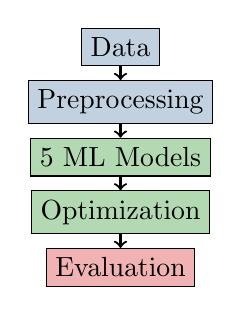
\begin{tikzpicture}[scale=0.7]
% ML Pipeline flowchart
\node[draw, rectangle, fill=lightblue!30] (data) at (0,4) {Data};
\node[draw, rectangle, fill=lightblue!30] (prep) at (0,3) {Preprocessing};
\node[draw, rectangle, fill=green!30] (models) at (0,2) {5 ML Models};
\node[draw, rectangle, fill=green!30] (opt) at (0,1) {Optimization};
\node[draw, rectangle, fill=red!30] (eval) at (0,0) {Evaluation};

\draw[->, thick] (data) -- (prep);
\draw[->, thick] (prep) -- (models);
\draw[->, thick] (models) -- (opt);
\draw[->, thick] (opt) -- (eval);
\end{tikzpicture}
\end{column}
\end{columns}
\end{frame}

\begin{frame}{Dataset Statistical Summary}
\begin{center}
\textbf{Battery Capacity Target Variable Statistics}
\end{center}

\vspace{0.3cm}
\begin{table}[h]
\centering
\begin{tabular}{@{}lc@{}}
\toprule
\textbf{Statistical Measure} & \textbf{Value} \\
\midrule
\textbf{Count} & 467 samples \\
\textbf{Capacity Mean} & 8,982.47 \\
\textbf{Capacity std} & 775.91 \\
\textbf{Min Capacity}  & 6,522.40 \\
\textbf{Max Capacity} & 10,027.01 \\
\textbf{Min Feature (abs)} & 6.36e-09 \\
\textbf{Max Feature (abs)} & 3.6e-02 \\

\bottomrule
\end{tabular}
\end{table}

\end{frame}

\begin{frame}{Data Preprocessing}
\begin{columns}
\begin{column}{0.6\textwidth}
\textbf{The Problem:}
\begin{itemize}
\item Different features have \textbf{different scales}
\item Impedance measurements vary widely in magnitude
\item ML algorithms are \textbf{sensitive to feature scales}
\item Distance-based algorithms especially affected
\end{itemize}

\vspace{0.3cm}
\textbf{Standardization Benefits:}
\begin{itemize}
\item \textbf{Equal feature importance} in distance calculations
\item \textbf{Faster convergence} for gradient-based algorithms
\item \textbf{Improved numerical stability}
\item \textbf{Better model performance} across different algorithms
\end{itemize}
\end{column}
\begin{column}{0.4\textwidth}
\begin{block}{Z-Score Standardization}
$$z = \frac{x - \mu}{\sigma}$$

Where:
\begin{itemize}
\item $x$ = original value
\item $\mu$ = mean
\item $\sigma$ = standard deviation
\item $z$ = standardized value
\end{itemize}
\end{block}

\vspace{0.2cm}
\begin{alertblock}{Result}
All features have:
\begin{itemize}
\item Mean = 0
\item Std Dev = 1
\end{itemize}
\end{alertblock}
\end{column}
\end{columns}
\end{frame}



\begin{frame}{Cross-Validation \& Model Selection}
\begin{columns}
\begin{column}{0.6\textwidth}
\textbf{Model Comparison Results:}
\begin{itemize}
\item \textbf{Random Forest:} Best overall performance
\item \textbf{Cross-validation score:} 0.8133
\item \textbf{Consistent performance} across different data splits
\item \textbf{Superior to linear models} due to non-linear relationships
\end{itemize}

\vspace{0.3cm}
\textbf{Key Insights:}
\begin{itemize}
\item Complex impedance-capacity relationships
\item Feature interactions are important
\item Ensemble methods excel for this problem
\end{itemize}
\end{column}
\begin{column}{0.4\textwidth}
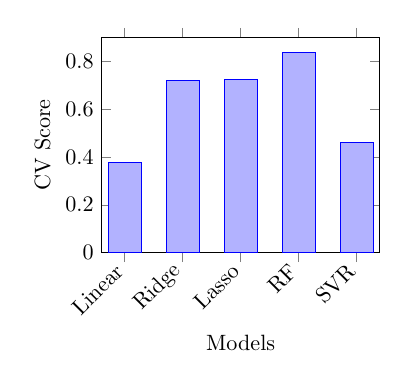
\begin{tikzpicture}[scale=0.8]
% Performance comparison chart
\begin{axis}[
    ybar,
    bar width=15pt,
    ylabel={CV Score},
    xlabel={Models},
    ymin=0,
    ymax=0.9,
    symbolic x coords={Linear,Ridge,Lasso,RF,SVR},
    xtick=data,
    x tick label style={rotate=45,anchor=east},
    width=6cm,
    height=5cm
]
\addplot coordinates {
    (Linear,0.3751)
    (Ridge,0.7213)
    (Lasso,0.7236)
    (RF,0.8387)
    (SVR,0.4590)
};
\end{axis}
\end{tikzpicture}
\end{column}

\end{columns}
\end{frame}

\section{Results \& Performance}

\begin{frame}{Model Performance Results}
\begin{center}
\textbf{Best Performing Model: Random Forest (Optimized)}
\end{center}

\vspace{0.3cm}
\begin{table}[h]
\centering
\begin{tabular}{@{}lccc@{}}
\toprule
\textbf{Metric} & \textbf{Training Set} & \textbf{Test Set} & \textbf{Difference} \\
\midrule
\textbf{R² Score} & \textcolor{green}{0.9173} & \textcolor{green}{\textbf{0.8798}} & -0.0375 \\
\textbf{RMSE} & 225.99 & 252.99 & -27.00 \\
\textbf{MAE} & 156.27 & 172.92 & -16.65 \\
\textbf{MSE} & 51,070.91 & 64,004.72 & -12,933.81 \\
\bottomrule
\end{tabular}
\end{table}

\vspace{0.5cm}
\begin{alertblock}{Key Performance Insights}
\begin{itemize}
\item \textbf{88\% variance explained} on test set - excellent predictive power
\item \textbf{Minimal overfitting} - good generalization capability
\item \textbf{RMSE of ~253 units} - practically acceptable prediction error
\end{itemize}
\end{alertblock}
\end{frame}

\begin{frame}{Classification Performance}
\begin{columns}
\begin{column}{0.5\textwidth}
\textbf{5-Bin Classification System:}
\begin{itemize}
\item \textbf{Bin 1:} $\leq$ 7,000 (Poor)
\item \textbf{Bin 2:} 7,000 -- 7,400 (Fair)
\item \textbf{Bin 3:} 7,400 -- 8,000 (Good)
\item \textbf{Bin 4:} 8,000 -- 8,500 (Very Good)
\item \textbf{Bin 5:} $>$ 8,500 (Excellent)
\end{itemize}
\end{column}
\begin{column}{0.5\textwidth}
\begin{table}[h]
\centering
\small
\begin{tabular}{@{}lcc@{}}
\toprule
\textbf{Metric} & \textbf{Training} & \textbf{Test} \\
\midrule
\textbf{Accuracy} & 89.54\% & \textcolor{green}{\textbf{91.49\%}} \\
\textbf{F1 (Weighted)} & 88.47\% & \textcolor{green}{\textbf{91.34\%}} \\
\textbf{F1 (Macro)} & 64.50\% & 79.42\% \\
\textbf{Cohen's Kappa} & 0.8642 & \textcolor{green}{\textbf{0.8891}} \\
\bottomrule
\end{tabular}
\end{table}
\end{column}
\end{columns}

\vspace{0.5cm}
\begin{block}{Classification Success}
\textbf{91.49\% accuracy} demonstrates excellent capability for battery health assessment and practical decision-making.
\end{block}
\end{frame}

\begin{frame}{Cohen's Kappa: Advanced Classification Metric}
\begin{columns}
\begin{column}{0.6\textwidth}
\textbf{What is Cohen's Kappa?}
\begin{itemize}
\item Measures \textbf{agreement beyond chance}
\item Accounts for \textbf{class imbalance}
\item More robust than simple accuracy
\item Values range from -1 to +1
\end{itemize}

\vspace{0.3cm}
\textbf{Formula:}
$$\kappa = \frac{p_o - p_e}{1 - p_e}$$

Where:
\begin{itemize}
\item $p_o$ = observed agreement (accuracy)
\item $p_e$ = expected agreement by chance
\end{itemize}

\vspace{0.3cm}
\textbf{Our Result: $\kappa = 0.8891$}
\begin{itemize}
\item \textcolor{green}{\textbf{Excellent agreement}} (0.81-1.00)
\item Much better than chance
\end{itemize}
\end{column}
\begin{column}{0.4\textwidth}
\textbf{Interpretation Scale:}
\begin{table}[h]
\centering
\small
\begin{tabular}{@{}ll@{}}
\toprule
\textbf{Kappa} & \textbf{Agreement} \\
\midrule
< 0.00 & Poor \\
0.00-0.20 & Slight \\
0.21-0.40 & Fair \\
0.41-0.60 & Moderate \\
0.61-0.80 & Substantial \\
\textcolor{green}{\textbf{0.81-1.00}} & \textcolor{green}{\textbf{Excellent}} \\
\bottomrule
\end{tabular}
\end{table}

\vspace{0.3cm}
\textbf{Test Set Per-Bin Results:}
\begin{table}[h]
\centering
\tiny
\begin{tabular}{@{}lcc@{}}
\toprule
\textbf{Bin} & \textbf{Precision} & \textbf{Recall} \\
\midrule
Bin 1 & 0.67 & 0.67 \\
Bin 2 & 0.75 & 0.75 \\
Bin 3 & 0.69 & 0.69 \\
Bin 4 & 0.97 & 0.97 \\
Bin 5 & 0.98 & 0.98 \\
\bottomrule
\end{tabular}
\end{table}
\end{column}
\end{columns}
\end{frame}

\begin{frame}{Grid Search Hyperparameter Optimization}
\begin{columns}
\begin{column}{0.5\textwidth}
\textbf{Random Forest Parameters Tuned:}
\begin{table}[h]
\centering
\small
\begin{tabular}{@{}ll@{}}
\toprule
\textbf{Parameter} & \textbf{Values Tested} \\
\midrule
n\_estimators & [50, 100, 200] \\
max\_depth & [10, 20, None] \\
min\_samples\_split & [2, 5, 10] \\
min\_samples\_leaf & [1, 2, 4] \\
\bottomrule
\end{tabular}
\end{table}

\vspace{0.3cm}
\textbf{Grid Search Configuration:}
\begin{itemize}
\item \textbf{Total combinations:} 81 parameter sets
\item \textbf{Cross-validation:} 4-fold CV
\item \textbf{Scoring metric:} R² score
\item \textbf{Best score achieved:} 0.8133
\end{itemize}
\end{column}
\begin{column}{0.5\textwidth}
\textbf{Parameter Definitions:}

\begin{block}{n\_estimators}
Number of decision trees in the forest. More trees generally improve performance but increase computation time.
\end{block}

\begin{block}{max\_depth}
Maximum depth of each tree. Controls model complexity and overfitting. None = unlimited depth.
\end{block}

\begin{block}{min\_samples\_split}
Minimum samples required to split an internal node. Higher values prevent overfitting.
\end{block}

\begin{block}{min\_samples\_leaf}
Minimum samples required at each leaf node. Smooths the model and prevents overfitting.
\end{block}
\end{column}
\end{columns}
\end{frame}



\section{Code Structure}

\begin{frame}{Technical Architecture}
\begin{center}
\textbf{Modular Python Implementation}
\end{center}

\vspace{0.3cm}
\begin{columns}
\begin{column}{0.5\textwidth}
\textbf{Core Modules:}
\begin{itemize}
\item \texttt{data\_loader.py}: Data ingestion
\item \texttt{preprocessor.py}: Feature engineering
\item \texttt{model\_trainer.py}: ML algorithms
\item \texttt{evaluator.py}: Performance assessment
\end{itemize}
\end{column}
\begin{column}{0.5\textwidth}
\textbf{Key Features:}
\begin{itemize}
\item Clean, maintainable code
\item Reproducible research approach
\item Comprehensive documentation
\item Production-ready deployment
\end{itemize}
\end{column}
\end{columns}

\vspace{0.5cm}
\begin{block}{Deliverables}
\begin{itemize}
\item Optimized model artifacts (saved as \texttt{.joblib} files)
\item Comprehensive analysis notebook
\item Performance visualization plots
\item Complete project documentation
\end{itemize}
\end{block}
\end{frame}

\section{Conclusions}

\begin{frame}{Key Achievements}
\begin{center}
\Large \textbf{Project Success Metrics}
\end{center}

\vspace{0.5cm}
\begin{columns}
\begin{column}{0.5\textwidth}
\begin{block}{Regression Performance}
\begin{itemize}
\item[\checkmark] \textbf{88\% R² Score} on test data
\item[\checkmark] \textbf{RMSE: 253 units} - practical accuracy
\item[\checkmark] \textbf{Strong generalization} capability
\item[\checkmark] \textbf{Minimal overfitting} observed
\end{itemize}
\end{block}
\end{column}
\begin{column}{0.5\textwidth}
\begin{block}{Classification Performance}
\begin{itemize}
\item[\checkmark] \textbf{91\% Classification accuracy}
\item[\checkmark] \textbf{Robust health assessment}
\item[\checkmark] \textbf{Production-ready model}
\item[\checkmark] \textbf{Real-world applicability}
\end{itemize}
\end{block}
\end{column}
\end{columns}

\vspace{0.5cm}
\begin{alertblock}{Overall Impact}
Successfully developed a \textbf{non-destructive, high-accuracy battery capacity prediction system} suitable for industrial deployment.
\end{alertblock}
\end{frame}



\section{Questions \& Discussion}

\begin{frame}{Thank You!}

\vspace{1cm}
\begin{center}
\Large \textcolor{darkblue}{\textbf{Questions \& Discussion}}
\end{center}
\end{frame}

\end{document}
